\begin{figure}[H]
    \centering
    \tikzset{every picture/.style={line width=0.75pt}} %set default line width to 0.75pt        
    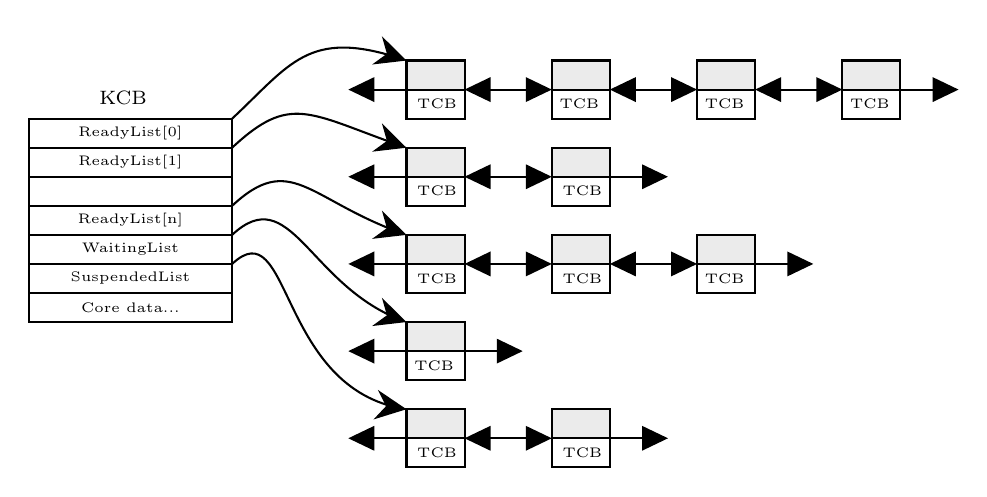
\begin{tikzpicture}[x=0.75pt,y=0.75pt,yscale=-1,xscale=1, scale=1.4]
        
        \foreach \x in {30,40,...,80}{
            \draw   (70,\x) -- (140,\x) -- (140,\x+10) -- (70,\x+10) -- cycle ;
        }
        
        \draw   (70,90) -- (140,90) -- (140,100) -- (70,100) -- cycle ;
        \draw   (200,10) -- (220,10) -- (220,30) -- (200,30) -- cycle ;
        \draw   (250,10) -- (270,10) -- (270,30) -- (250,30) -- cycle ;
        \draw  [fill=lightgray!50  ,fill opacity=0.62 ] (200,10) -- (220,10) -- (220,20) -- (200,20) -- cycle ;
        \draw  [fill=lightgray!50  ,fill opacity=0.62 ] (250,10) -- (270,10) -- (270,20) -- (250,20) -- cycle ;
        \draw    (223,20) -- (247,20) ;
        \draw [shift={(250,20)}, rotate = 180] [fill=black  ][line width=0.08]  [draw opacity=0] (8.93,-4.29) -- (0,0) -- (8.93,4.29) -- cycle    ;
        \draw [shift={(220,20)}, rotate = 0] [fill=black  ][line width=0.08]  [draw opacity=0] (8.93,-4.29) -- (0,0) -- (8.93,4.29) -- cycle    ;
        \draw   (300,10) -- (320,10) -- (320,30) -- (300,30) -- cycle ;
        \draw   (350,10) -- (370,10) -- (370,30) -- (350,30) -- cycle ;
        \draw  [fill=lightgray!50  ,fill opacity=0.62 ] (300,10) -- (320,10) -- (320,20) -- (300,20) -- cycle ;
        \draw  [fill=lightgray!50  ,fill opacity=0.62 ] (350,10) -- (370,10) -- (370,20) -- (350,20) -- cycle ;
        \draw    (323,20) -- (347,20) ;
        \draw [shift={(350,20)}, rotate = 180] [fill=black  ][line width=0.08]  [draw opacity=0] (8.93,-4.29) -- (0,0) -- (8.93,4.29) -- cycle    ;
        \draw [shift={(320,20)}, rotate = 0] [fill=black  ][line width=0.08]  [draw opacity=0] (8.93,-4.29) -- (0,0) -- (8.93,4.29) -- cycle    ;
        \draw    (273,20) -- (297,20) ;
        \draw [shift={(300,20)}, rotate = 180] [fill=black  ][line width=0.08]  [draw opacity=0] (8.93,-4.29) -- (0,0) -- (8.93,4.29) -- cycle    ;
        \draw [shift={(270,20)}, rotate = 0] [fill=black  ][line width=0.08]  [draw opacity=0] (8.93,-4.29) -- (0,0) -- (8.93,4.29) -- cycle    ;
        \draw    (370,20) -- (387,20) ;
        \draw [shift={(390,20)}, rotate = 180] [fill=black  ][line width=0.08]  [draw opacity=0] (8.93,-4.29) -- (0,0) -- (8.93,4.29) -- cycle    ;
        \draw    (200,20) -- (183,20) ;
        \draw [shift={(180,20)}, rotate = 360] [fill=black  ][line width=0.08]  [draw opacity=0] (8.93,-4.29) -- (0,0) -- (8.93,4.29) -- cycle    ;
        \draw    (140,30) .. controls (159.99,11.34) and (166.19,-0.95) .. (197.54,9.18) ;
        \draw [shift={(200,10)}, rotate = 199.06] [fill=black  ][line width=0.08]  [draw opacity=0] (10.72,-5.15) -- (0,0) -- (10.72,5.15) -- (7.12,0) -- cycle    ;
        \draw   (200,40) -- (220,40) -- (220,60) -- (200,60) -- cycle ;
        \draw   (250,40) -- (270,40) -- (270,60) -- (250,60) -- cycle ;
        \draw  [fill=lightgray!50  ,fill opacity=0.62 ] (200,40) -- (220,40) -- (220,50) -- (200,50) -- cycle ;
        \draw  [fill=lightgray!50  ,fill opacity=0.62 ] (250,40) -- (270,40) -- (270,50) -- (250,50) -- cycle ;
        \draw    (223,50) -- (247,50) ;
        \draw [shift={(250,50)}, rotate = 180] [fill=black  ][line width=0.08]  [draw opacity=0] (8.93,-4.29) -- (0,0) -- (8.93,4.29) -- cycle    ;
        \draw [shift={(220,50)}, rotate = 0] [fill=black  ][line width=0.08]  [draw opacity=0] (8.93,-4.29) -- (0,0) -- (8.93,4.29) -- cycle    ;
        \draw    (270,50) -- (287,50) ;
        \draw [shift={(290,50)}, rotate = 180] [fill=black  ][line width=0.08]  [draw opacity=0] (8.93,-4.29) -- (0,0) -- (8.93,4.29) -- cycle    ;
        \draw    (200,50) -- (183,50) ;
        \draw [shift={(180,50)}, rotate = 360] [fill=black  ][line width=0.08]  [draw opacity=0] (8.93,-4.29) -- (0,0) -- (8.93,4.29) -- cycle    ;
        \draw    (140,40) .. controls (159.99,21.34) and (166.19,28.07) .. (197.54,39.14) ;
        \draw [shift={(200,40)}, rotate = 199.06] [fill=black  ][line width=0.08]  [draw opacity=0] (10.72,-5.15) -- (0,0) -- (10.72,5.15) -- (7.12,0) -- cycle    ;
        \draw   (200,70) -- (220,70) -- (220,90) -- (200,90) -- cycle ;
        \draw   (250,70) -- (270,70) -- (270,90) -- (250,90) -- cycle ;
        \draw  [fill=lightgray!50  ,fill opacity=0.62 ] (200,70) -- (220,70) -- (220,80) -- (200,80) -- cycle ;
        \draw  [fill=lightgray!50  ,fill opacity=0.62 ] (250,70) -- (270,70) -- (270,80) -- (250,80) -- cycle ;
        \draw    (223,80) -- (247,80) ;
        \draw [shift={(250,80)}, rotate = 180] [fill=black  ][line width=0.08]  [draw opacity=0] (8.93,-4.29) -- (0,0) -- (8.93,4.29) -- cycle    ;
        \draw [shift={(220,80)}, rotate = 0] [fill=black  ][line width=0.08]  [draw opacity=0] (8.93,-4.29) -- (0,0) -- (8.93,4.29) -- cycle    ;
        \draw    (200,80) -- (183,80) ;
        \draw [shift={(180,80)}, rotate = 360] [fill=black  ][line width=0.08]  [draw opacity=0] (8.93,-4.29) -- (0,0) -- (8.93,4.29) -- cycle    ;
        \draw    (140,60) .. controls (159.99,41.34) and (166.19,57.57) .. (197.54,69.12) ;
        \draw [shift={(200,70)}, rotate = 199.06] [fill=black  ][line width=0.08]  [draw opacity=0] (10.72,-5.15) -- (0,0) -- (10.72,5.15) -- (7.12,0) -- cycle    ;
        \draw    (273,80) -- (297,80) ;
        \draw [shift={(300,80)}, rotate = 180] [fill=black  ][line width=0.08]  [draw opacity=0] (8.93,-4.29) -- (0,0) -- (8.93,4.29) -- cycle    ;
        \draw [shift={(270,80)}, rotate = 0] [fill=black  ][line width=0.08]  [draw opacity=0] (8.93,-4.29) -- (0,0) -- (8.93,4.29) -- cycle    ;
        \draw   (300,70) -- (320,70) -- (320,90) -- (300,90) -- cycle ;
        \draw  [fill=lightgray!50  ,fill opacity=0.62 ] (300,70) -- (320,70) -- (320,80) -- (300,80) -- cycle ;
        \draw    (320,80) -- (337,80) ;
        \draw [shift={(340,80)}, rotate = 180] [fill=black  ][line width=0.08]  [draw opacity=0] (8.93,-4.29) -- (0,0) -- (8.93,4.29) -- cycle    ;
        \draw   (200,100) -- (220,100) -- (220,120) -- (200,120) -- cycle ;
        \draw  [fill=lightgray!50  ,fill opacity=0.62 ] (200,100) -- (220,100) -- (220,110) -- (200,110) -- cycle ;
        \draw    (220,110) -- (237,110) ;
        \draw [shift={(240,110)}, rotate = 180] [fill=black  ][line width=0.08]  [draw opacity=0] (8.93,-4.29) -- (0,0) -- (8.93,4.29) -- cycle    ;
        \draw    (200,110) -- (183,110) ;
        \draw [shift={(180,110)}, rotate = 360] [fill=black  ][line width=0.08]  [draw opacity=0] (8.93,-4.29) -- (0,0) -- (8.93,4.29) -- cycle    ;
        \draw    (140,70) .. controls (159.99,51.34) and (166.19,86.59) .. (197.54,99.08) ;
        \draw [shift={(200,100)}, rotate = 199.06] [fill=black  ][line width=0.08]  [draw opacity=0] (10.72,-5.15) -- (0,0) -- (10.72,5.15) -- (7.12,0) -- cycle    ;
        \draw   (200,130) -- (220,130) -- (220,150) -- (200,150) -- cycle ;
        \draw   (250,130) -- (270,130) -- (270,150) -- (250,150) -- cycle ;
        \draw  [fill=lightgray!50  ,fill opacity=0.62 ] (200,130) -- (220,130) -- (220,140) -- (200,140) -- cycle ;
        \draw  [fill=lightgray!50  ,fill opacity=0.62 ] (250,130) -- (270,130) -- (270,140) -- (250,140) -- cycle ;
        \draw    (223,140) -- (247,140) ;
        \draw [shift={(250,140)}, rotate = 180] [fill=black  ][line width=0.08]  [draw opacity=0] (8.93,-4.29) -- (0,0) -- (8.93,4.29) -- cycle    ;
        \draw [shift={(220,140)}, rotate = 0] [fill=black  ][line width=0.08]  [draw opacity=0] (8.93,-4.29) -- (0,0) -- (8.93,4.29) -- cycle    ;
        \draw    (270,140) -- (287,140) ;
        \draw [shift={(290,140)}, rotate = 180] [fill=black  ][line width=0.08]  [draw opacity=0] (8.93,-4.29) -- (0,0) -- (8.93,4.29) -- cycle    ;
        \draw    (200,140) -- (183,140) ;
        \draw [shift={(180,140)}, rotate = 360] [fill=black  ][line width=0.08]  [draw opacity=0] (8.93,-4.29) -- (0,0) -- (8.93,4.29) -- cycle    ;
        \draw    (140,80) .. controls (160.09,61.24) and (155.69,120.96) .. (197.39,129.54) ;
        \draw [shift={(200,130)}, rotate = 188.4] [fill=black  ][line width=0.08]  [draw opacity=0] (10.72,-5.15) -- (0,0) -- (10.72,5.15) -- (7.12,0) -- cycle    ;
        \draw (105,75) node  [font=\tiny] [align=left] {WaitingList};
        \draw (105,85) node  [font=\tiny] [align=left] {SuspendedList};
        \draw (105,35) node  [font=\tiny] [align=left] {ReadyList[0]};
        \draw (105,45) node  [font=\tiny] [align=left] {ReadyList[1]};
        \draw (105,65) node  [font=\tiny] [align=left] {ReadyList[n]};
        \draw (105,95) node  [font=\tiny] [align=left] {Core data...};
        \draw (102.5,23) node  [font=\scriptsize] [align=left] {KCB};
        \draw (210.5,25) node  [font=\tiny] [align=left] {TCB};
        \draw (259.5,25) node  [font=\tiny] [align=left] {TCB};
        \draw (309.5,25) node  [font=\tiny] [align=left] {TCB};
        \draw (359.5,25) node  [font=\tiny] [align=left] {TCB};
        \draw (210.5,55) node  [font=\tiny] [align=left] {TCB};
        \draw (260.5,55) node  [font=\tiny] [align=left] {TCB};
        \draw (210.5,85) node  [font=\tiny] [align=left] {TCB};
        \draw (260.5,85) node  [font=\tiny] [align=left] {TCB};
        \draw (309.5,85) node  [font=\tiny] [align=left] {TCB};
        \draw (209.5,115) node  [font=\tiny] [align=left] {TCB};
        \draw (210.5,145) node  [font=\tiny] [align=left] {TCB};
        \draw (260.5,145) node  [font=\tiny] [align=left] {TCB};
    \end{tikzpicture}
    \caption{OS lists}
    \label{fig:corelists}
\end{figure}